\subsection{Data}
\label{back:data}

\subsubsection{Normalization and Standardization}

Normalization is a technique of which data is transformed from it's original scale, to a more standard scale. These techniques are normally used when the dataset has elements of different ranges. Normalization contribute to faster convergence, and it's why they are as commonly used when preprocessing neural networks. 
The two most common types of normalization are minmax and z score. \\

\textbf{MinMax Normalization}

This algorithm transforms data to a specified range, most often $[0, 1]$ but it can also be $[-1, 1]$ or any other range.
Minmax normalization can be described as follows:

\begin{equation}
   x_{normalized} = \dfrac{x - x_{min}}{x_{max}-x_{min}}
\end{equation}

\textbf{ZScore Standardization}

Contrary to normalization, standardization aims to transform the values to have a mean of 0, and a standard deviation of 1. It also assumes a distribution close to that of a normal one. This method can be expressed as follows. \\ 
\begin{equation}
   x_{standardized} = \dfrac{x - \mu}{\sigma}
\end{equation}

\subsection{Half Precision Training}

Working with large datasets and \acrshort{dnn}s can be rather time- and resource consumptive. To address this, one can cast the datatype from single precision to half precision, along with weights, biases and activations. This will reduce in loss of accuracy and information, but it can drastically lower memory consumption and decrease training time. It is important to note that casting of data occurs with normalization techniques, the order of which operation happens first is quintessential. If the data is casted to half precision before normalization, the normalization will be based on a slightly inaccurate representation of the data, but the computation of the normalized data will be faster. If normalization were to occur first, less detail about the data would be lost, but at the expense of being more computational intensive. \\

\textbf{Mixed precision training}

Mixed precision training, introduced in 2018 \cite{micikevicius2018mixed}, is a technique where the weights, activations and biases of a neural network is stored in single precision, while the data itself stays in it's original format. It allows for reduced memory consumption, while also speeding up operations of deep neural nets. Additionally, the amount of $kwH$ required to train the neural nets would decrease, thus reducing both the cost and the environmental tax by training neural nets. This becomes more important the larger the datasets, models and the sheer amount of GPUS required to train massive workloads. This introduce the concept of loss scaling, where the losses needs to be adjusted based on the weights. \\

\subsection{Datasets}

Loading and processing data before it's trained is a crucial task of constructing any neural networks. In many of the most popular frameworks such as \texttt{Pytorch} and \texttt{TensorFlow}, Datasets and Dataloaders are used to retrieve data from a certain location, transform it to fit the network, and load the data in batches to the model. \\

Datasets are objects that contain information about where to gather the data from, which transformations are to be applied, and functions to gather a single instance of a batch.

\subsection{Dataloaders}

If the datasets contain information about the data and how to retrieve a single instance, the dataloaders job is to create an object that can be iterated over, containing $n$ amount of batches, and transferring these data to the wanted devices. In the case of data parallel multi-gpu training, when the data is loaded, it's \textit{sharded} across the different gpus, in a manner that balances the load of each gpu. Let's say we have a batch  of size $[4, 5, 5]$ and we have two gpus available. The dataloader can split this Tensor in two batches, where each of the gpus get a tensor of size $[2, 5, 5]$. By sharding the data along the first axis, ideally we can half the amount it takes, not taking data transfer time into consideration. 

\begin{figure}[h]
    \centering
    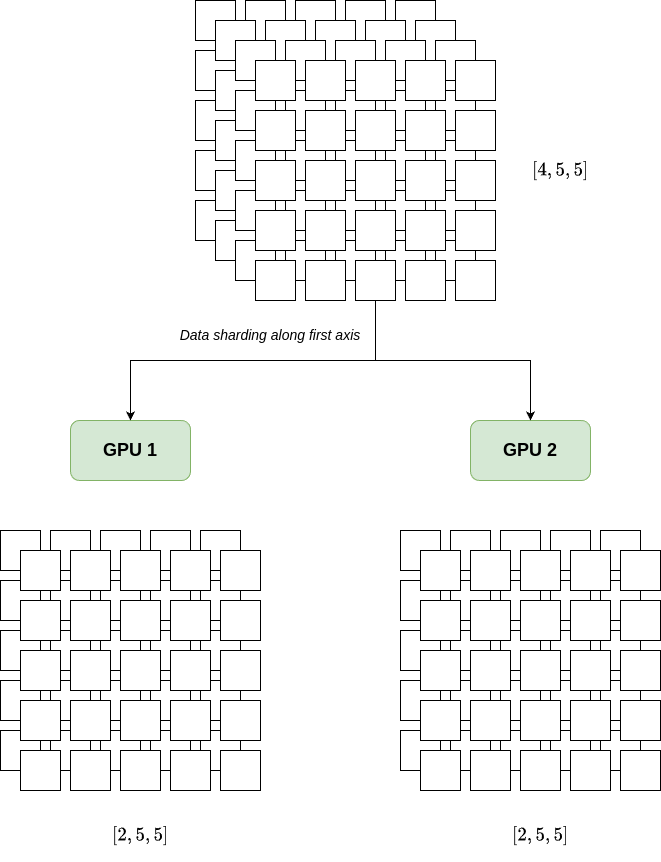
\includegraphics[scale=0.2]{figures/sharding.png}
    \caption{Example of data sharding with 2 gpus, and a original Tensor of size [4,5,5]}
    \label{fig:sharding}
\end{figure}


\textbf{Parallel loading}

When iterating over the dataloader, each element of the batch is retrieved and undergoes transformations. Depending on the batch size and  the size of the data, this procecedure can be very resource-intensice and time-consuming. To mitigate this, we can introduce the concept of parallel batch loading. Instead of gathering and transforming the data sequentially, we instead introduce several workers to be able to do this process in parallel. 

\lstinputlisting[language=Python]{code/parallel_batch_load.py}